\chapter{Treplica Reconfigurável}\label{cap2}

Descrever a proposta e sua implementação.

\section{Visão arquitetural de Treplica}

Introdução da arquitetura de treplica

\subsection{Componentes de suporte}

Comentar sobre a abstração dos componentes de suporte

\subsubsection{Transport}\label{subsec:transport}

\subsubsection{Change Log}

\subsubsection{Ledger}

Ledger é a abstração do estado persistente para implementação de Paxos. É uma estrutura
de dados comum, compartilhada por todos os agentes de Paxos, implementados por Treplica,
que conseguem através de uma interface acessar a memória principal. A implementação dessa
interface suporta persistência dos dados de forma não-volátil. Conforme definido no
\autoref{cap1:replicacao_ativa_paxos}, é possível obter o mesmo estado replicado a partir
das instâncias de consenso armazenadas em memória persistente. Assim, a abstração do
Ledger concentra todos os dados de uma instância de consenso bem sucedido em memória
persistente, facilmente acessível a partir da memória principal. A classe LoggingLedger é
o objeto utilizado para persistir em log (disco) as alterações. Para simplificar o uso de
log de alterações, esta implementação tem suporte para detectar e isolar as alterações
feitas em seu estado interno. Pode gravar mudanças no estado e depois recuperá-la,
reaplicando um conjunto de alterações previamente gravados. O Ledger armazena o estado
completo de cada instância do consenso por réplica, mantendo todos os dados exigidos por
todos os tipos de agentes de Paxos implementados por Treplica. Dessa forma, é possível que
qualquer agente recupere seu estado, inclusive o coordenador.

\subsubsection{Secretary}\label{subsec:secretary}

Secretary apresenta uma abstração unificada de I/O para os agentes de Paxos. Este
componente utiliza memória persistente usando \emph{change log} e o Ledger, lida com a
passagem de mensagens usando o componente de transporte e lida também com a fila de
objetos utilizada para entregar objetos para a aplicação. A principal razão para criação
dessa abstração em Treplica foi sintetizar as operações de I/O em \emph{threads}
diferentes das que executam as operações de Paxos. Operações de I/O em disco, tem grande
potencial para reduzir o desempenho do algoritmo Paxos por duas razões: (1) todas as
requisições de escrita que estabeleceram consenso, devem ser persistidas de forma
não-volátil antes do progresso do algoritmo. Premissa para garantir consistência; (2)
alguns passos do algoritmo de Paxos podem demandar muito acesso a memória persistente.
Considerando que cada operação de escrita em disco leva cerca de $1ms$ para ser concluída
e que uma rodada de Paxos, pelo menos, requer duas escritas em memória estável, acabamos
de adicionar uma latência de $2ms$ em todas as rodadas de consenso.

Uma vez que o I/O é tratado apenas pelo Secretary de forma assíncrona é possível resolver
o problema de falta de paralelismo entre as rodadas. Isso é feito através de uma fila de
agrupamento de gravações lógicas distintas que retém os dados realizar uma única gravação
física. Essa abordagem é vantajosa porque o tamanho dos dados de escrita no disco, utiliza
uma \emph{sync() system call} causando um pouco latência na operação. A implementação d
de Scretary absorve latência da \emph{system call} mantendo uma \emph{thread} separada
para persistência dos dados.

\subsubsection{Router}

Router é um componente simples, mas vital para PaxosPersistentQueue, porque inicia todos
os agentes em conjunto. Sua função principal é prover o \emph{main loop} da implementação
de Paxos, que recebe mensagens do componente de transporte e, de acordo com seu tipo,
encaminha para o agente apropriado. Dessa forma, a execução desse agente é sequencial e
compartilha estruturas de dados, como o Ledger, não precisa de controle de concorrência.

Esse é o único componente (\emph{thread}) que monitora o temporizador central e gera
eventos de \emph{timer} \footnote{Os eventos de \emph{timer} simbolizam a passagem do
tempo para a aplicação. Esse evento atinge todos os componentes que necessitam de um
relógio para seu correto funcionamento}. O código de processamento dos agentes não possuem
operações que geram grandes bloqueios, eles são programados como simples manipuladores de
eventos caracterizando uma arquitetura de processamento assíncrono baseada em eventos
(\emph{event-based}). É responsabilidade do Router instanciar agentes e componentes de
apoio e, também, inicializar a PaxosPersistentQueue.


\subsection{Componentes de Paxos}

Falar sobre a abstração dos componentes de Paxos

\subsubsection{Election}

\subsubsection{Learner}

\subsubsection{Coordinator}

Coordenador (\emph{coordinator}) é o agente responsável por conduzir a rodada de consenso.
Ele é capaz de decidir, através da aplicação de uma regra local, se uma rodada foi bem
sucedida ou não. A regra local do coordenador é baseada em quóruns de \emph{receptores} e
exige que pelo menos $\lfloor n/2 \rfloor + 1$ receptores façam parte de uma rodada, onde
$n$ é o número total de receptores na aplicação \cite{lamport98}.

É permitido a existência de apenas um coordenador por rodada, em caso de falha na réplica
que executa o agente coordenador, uma eleição de líder deve ser convocada para estabelecer
que uma réplica correta execute o agente coordenador. Como o algoritmo é executado no
modelo computacional falha-e-recuperação, a réplica defeituosa pode voltar a computação
acreditando que ainda é o coordenador. Nesse caso, uma nova eleição de líder deve ser
convocada novamente para restabelecer a unicidade de coordenador por rodada.

\subsubsection{Proposer}

Proponente (\emph{proposer}) são agentes capazes de propor valores. Os proponentes podem
propor dois valores diferentes concorrentemente (condição de concorrência)
\footnote{Também conhecida como condição de corrida, acontece quando diferentes processos
em execução atuam sobre um estado compartilhado \cite{alguem}}, nesse caso suas propostas
podem colidir inviabilizando o sucesso de uma rodada de consenso. Em caso de colisões,
diferentes mecanismos podem ser implementados, para lida com essa situação Treplica inicia
uma nova rodada por intermédio do agente \emph{coordenador}.

\subsubsection{Acceptor}

Colocar mais testo aqui!!!


\section{Alterações propostas}

Apresentamos, exaustivamente, os conceitos utilizados para criação da biblioteca Treplica,
os detalhes de seus componentes e como eles estão relacionados. A partir de agora, iremos
focar nossa discussão nas alterações propostas para expansão da biblioteca. O objetivo
dessa seção é a apresentar e detalhar as seguintes funcionalidades:

\begin{itemize}
  \item Protocolo para transferência de estado: mecanismo eficiente para transferência de
    estado entre réplicas.
  \item Réplicas leitoras: a ideia principal dessa abordagem é utilizar réplicas que não
    participam de processo de decisão de instâncias de consenso.
  \item Equalização de estado: proposta para novo componente que preenche lacunas na
    sequência de instâncias de consenso.
\end{itemize}

\subsection{Protocolo para transferência de estado}

A ideia principal dessa abordagem é a criação de um mecanismo que possibilite transferir, de
forma eficiente, o estado entre réplicas. Para isso, criamos um protocolo que orquestra as
iterações entre réplicas e os bloqueios de estado necessários para garantia de
consistência. Visando maior clareza de exposição, quando necessário, chamaremos as
réplicas que recebem o estado como \emph{réplicas receptoras} e réplicas que transferem
seu estado como \emph{réplicas doadoras}.

A necessidade de um mecanismo para transferência de estado surgiu a partir da suposição da
equalização de estados divergentes entre réplicas de um mesmo grupo. A disparidade de
estados em uma ambiente que emprega replicação ativa utilizando Paxos pode suceder a
partir de: (1) falha-e-recuperação de uma réplica. Durante o período defeituoso, uma
réplica pode perder $n$ decisões de consenso criando uma grande lacuna entre seu estado
recuperado e o estado corrente da aplicação; ou (2) a divergência de estados pode ter um
motivo mais nobre: expansão do aglomerado. No entanto, segundo \citeonline{lamport10},
toda operação para adição de réplica em Paxos deve ser precedida de uma operação não
trivial de reconfiguração.

Independente da motivação para aplicação de uma transferência de estado, essa operação
não deve gerar grande impacto para o processamento em grupo e deve preservar a correção do
algoritmo. Tendo em vista a garantia de consistência, implementamos essa operação como uma
tarefa \emph{síncrona} \footnote{No modelo requisição/resposta, o emissor dos dados fica
bloqueado até receber uma resposta do receptor \cite{coulouris11}}. As seguintes premissas
foram supostas para construção do protocolo:

\begin{itemize}
  \item Quando uma réplica inicia o processo de transferência, todas as mensagens
    recebidas não pertencentes ao protocolo de transferência devem ser ignoradas.
  \item A réplica doadora não deve processar nenhuma operação de escrita enquanto realiza
    a transferência de estado.
  \item Novas réplicas estarão aptas para processar requisições (leitura ou escrita)
    somente após a configuração de um estado inicial.
\end{itemize}

Baseado nessas premissas, podemos afirmar que a operação de transferência de estado é
custosa para o desempenho de Paxos, pois estamos bloqueando, temporariamente, a
participação de uma réplica no processo de decisão de instâncias de consenso.

\subsubsection{Funcionamento do protocolo}

Estabelecemos a premissa que é responsabilidade da réplica receptora encontrar uma réplica
doadora (réplica disposta a transferir o seu estado). A elegância do mecanismo de seleção
de doador é herdada de Treplica: as réplicas conhecem somente seu próprio identificador de
rede e podem alcançar todas as outras réplicas por uma primitiva simples de difusão.
Criamos o protocolo com a preocupação de minimizar a degradação de desempenho causada pela
operação de transferência de estado. Ele foi dividido em três fases, conforme ilustra a
\autoref{fig:fases_protocolo}.

\begin{itemize}
  \item Na Fase 1 (\emph{Fase de Negociação}) a réplica receptora envia uma mensagem com
    as regras do estado almejado (política contratual).
  \item Na Fase 2 (\emph{Seleção de Doadora}), ocorre a apuração do melhor acordo proposto
    pelas réplicas que atendem as exigências estabelecidas pela réplica receptora. Somente
    uma réplica doadora é selecionada.
  \item Finalmente, na Fase 3 (\emph{Transferência}) o estado da réplica doadora eleita na
    Fase 2 é transferido para a réplica receptora.
\end{itemize}

\begin{figure}[ht]
  \centering
  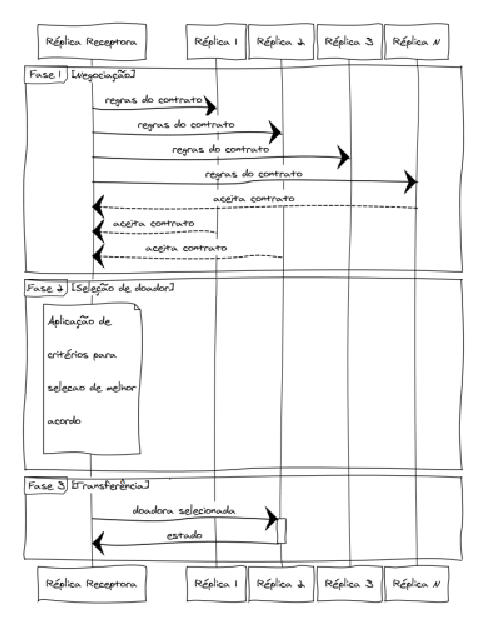
\includegraphics[width=11cm]{conteudo/capitulos/figuras/fases_protocolo.eps}
  \caption{Fases do protocolo de transferência de estado}
  \label{fig:fases_protocolo}
\end{figure}

Na Fase de Negociação, fase inicial, a réplica receptora estabelece as regras da
transferência de estado através da mensagem \classname{PolicyMessage}. Por exemplo,
supomos que, independente do motivo, uma réplica $r$ deseje receber um estado a partir da
instância de consenso $240$. Então, $r$ inicia a negociação de estado difundindo a
mensagem contratual. As réplicas que recebem essa mensagem de solicitação de negociação de
estado são solidárias e tentam atender essa requisição. Elas avaliam as exigências
contidas na mensagem e, caso estejam de acordo, enviam, somente para a replica receptora
(remetente do contrato), a mensagem \classname{DealMessage}. Essa proposta acordo, contém
informações referentes ao estado que a réplica doadora está oferecendo.

Caso a réplica receptora não receba nenhuma proposta de acordo após um tempo
pré-estabelecido, ela reinicia a Fase de Negociação até encontrar uma réplica doadora.
Podemos nos beneficiar desse \emph{loop} inicial que se encontra a réplica receptora para
criarmos diferentes políticas contratuais para transferência de estado. Nessa versão
proposta de Treplica, supomos configurações de duas politicas: uma mais agressiva e outra
mais ingênua. Lembrando que todas as políticas devem fornecer qual é a instância de
consenso pretendida.

\begin{itemize}
  \item Somente réplicas leitoras: essa política é mais restritiva, busca um acordo com
    uma réplica leitora \footnote{Réplicas leitoras são aquelas onde apenas os agentes
    proponente e aprendiz estão em execução. Elas não assumem um papel fundamental na
    execução de Paxos. Trataremos réplicas leitoras na \autoref{sec:replicas_leitoras}.
    Acordos com réplica leitoras são preferíveis devido à restrição de sincronia exigida
    pelo protocolo. Dessa forma, essa política tenta minimizar possíveis impactos na
    computação de Paxos.
  \item Qualquer réplica: essa política é a menos restritiva possível, busca um acordo
    independente da configuração da réplica.
\end{itemize}

Devemos ter cuidado ao eleger uma réplica votante como réplica doadora, pois podemos gerar
impacto direto no desempenho da aplicação. A réplica doadora não participará da eleição de
um novo estado durante o período que está transmitindo seu estado (congelamento do estado
para garantia de consistência). Lembrando que, no algoritmo Paxos, a partir do momento em
que a maioria dos receptores concordam com a alteração do estado, mais cedo ou mais tarde
todas as réplicas chegarão ao mesmo estado. A partir do momento que retiramos
temporariamente da computação uma réplica votante, a probabilidade de atingir consenso
pela maioria diminui, podendo até impossibilitar o progresso do algoritmo.

O protocolo progride quando a réplica receptora possui propostas de acordo. Quando essa
condição é alcançada, ela inicia a Fase de Seleção de Doadora. Fase que executa um
algoritmo simples capaz de eleger a réplica que propôs o melhor acordo. Somente a partir
do momento que o algoritmo estabelece uma réplica doadora a Fase de Transferência inicia.
Para a execução dessa fase, os seguintes aspectos de Treplica foram considerados: (1) o
estado de uma aplicação pode ser tão grande quanto a capacidade de memória de uma réplica;
(2) todas as mensagens são trocadas utilizando o protocolo UDP.

Optamos então pela utilização do protocolo TCP para transferência de estado cobiçando
maior vazão dos dados nessa operação. Somente o estado é enviado via TCP, todas as outras
mensagens pertencentes ao protocolo utilizam comunicação UDP, nativa de Treplica. Sendo
assim, a réplica receptora abre um \emph{socket} TCP e envia a mensagem
\classname{GETMessage} para a réplica doadora com o endereço do \emph{socket} TCP
recentemente aberto. Por sua vez, a réplica doadora bloqueia suas atividades e estabelece
a conexão TCP com a réplica leitora. Finalmente a transferência de estado é executada.

Assim que a operação é concluída, a conexão TCP entre as réplicas é finalizada. A réplica
doadora volta para computação e a réplica leitora começa a processar as requisições
encaminhadas pelos seus clientes. Estabelecemos um \emph{timeout} para evitar bloqueios
indevidos por falha em alguma das réplicas envolvidas na transação. Caso todas as etapas
do protocolo não sejam concluídas em no máximo 10 segundos, a negociação de estado é
reiniciada até que se obtenha êxito. A \autoref{fig:protocolo} ilustra o funcionamento do
protocolo com suas respectivas trocas de mensagens.

\begin{figure}[ht]
  \centering
  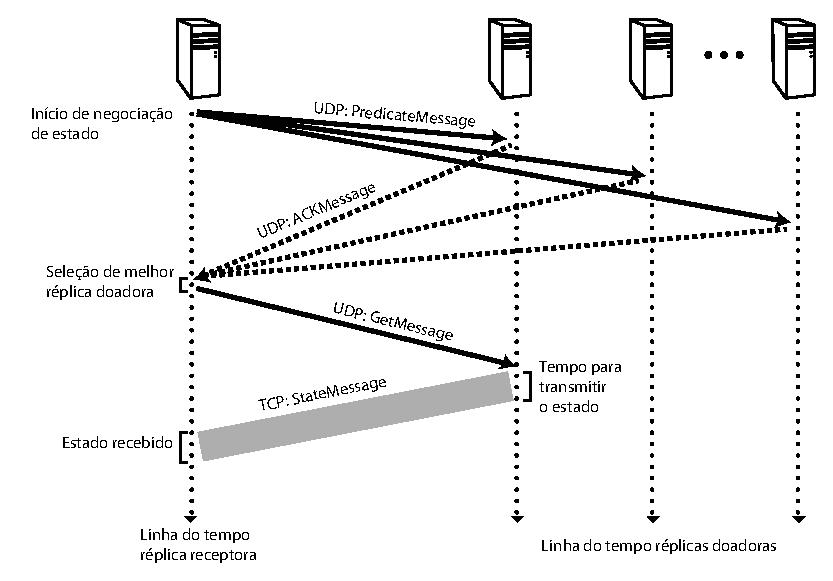
\includegraphics[width=11cm]{conteudo/capitulos/figuras/transferencia_estado.eps}
  \caption{Protocolo de transferência de estado}
  \label{fig:protocolo}
\end{figure}

\subsubsection{Componentes alterados}

Todas as classes de mensagem implementam a interface de marcação
\classname{StateTransferMessage}.

\subsubsubsection{PolicyMessage}

A classe \classname{PolicyMessage} é a primeira mensagem do protocolo para transferência
de estado. Essa classe além de sinalizar para as outras réplicas o interesse existente de
uma réplica em receber um estado, contém todas as informações sobre o estado pretendido
pela réplica receptora. Os dados contratuais são abstraídos pela classe
\classname{Policy}. Essa classe por sua vez, contém o número da instância de consenso
desejado e uma lista de regras que uma réplica deve obedecer para ser uma doadora.

\subsubsubsection{DealMessage}

A classe \classname{DealMessage} também pertence ao grupo de mensagens trocadas para
transferência de estado. Essa classe abstrai uma proposta de acordo para transferir
estado. Ela e uma sinalização para a réplica receptora, informa que existe uma réplica
disposta a ser doadora do estado e que atende todas as exigências do contrato.

Quanto mais mensagens propondo acordo na transferência a réplica receptora receber, menos
restritivas são suas exigências e maior a chance de selecionar uma réplica votante.

\subsubsubsection{GetMessage}

Descrever todos os componentes alterados para a utilização desse mecanismo.

\subsubsubsection{StateMessage}

Descrever todos os componentes alterados para a utilização desse mecanismo.

\subsubsubsection{Diplomat}

Descrever todos os componentes alterados para a utilização desse mecanismo.

\subsubsection{Política de Reconfiguração}

Primeiramente, estamos interessados em transferir estado quando trabalhamos com operações
de expansão em um aglomerado (\autoref{fig:inclusao}). Alguns aspecto precisam ser
considerados: (1) o estado da nova réplica está defasado com relação ao estado das
réplicas participantes do grupo. É imprescindível que essa defasagem seja suprimida; (2) a
operação de equiparação de estados deve gerar estados consistente; (3) o impacto gerado
para o processamento do aglomerado deve ser mínimo. Para justificar a inclusão de uma nova
réplica, obrigatoriamente é preciso geração de benefícios para o processamento em grupo,
caso contrário estamos executando operações sem serventia com potencial para saturar o
sistema.

\begin{figure}[ht]
  \centering
  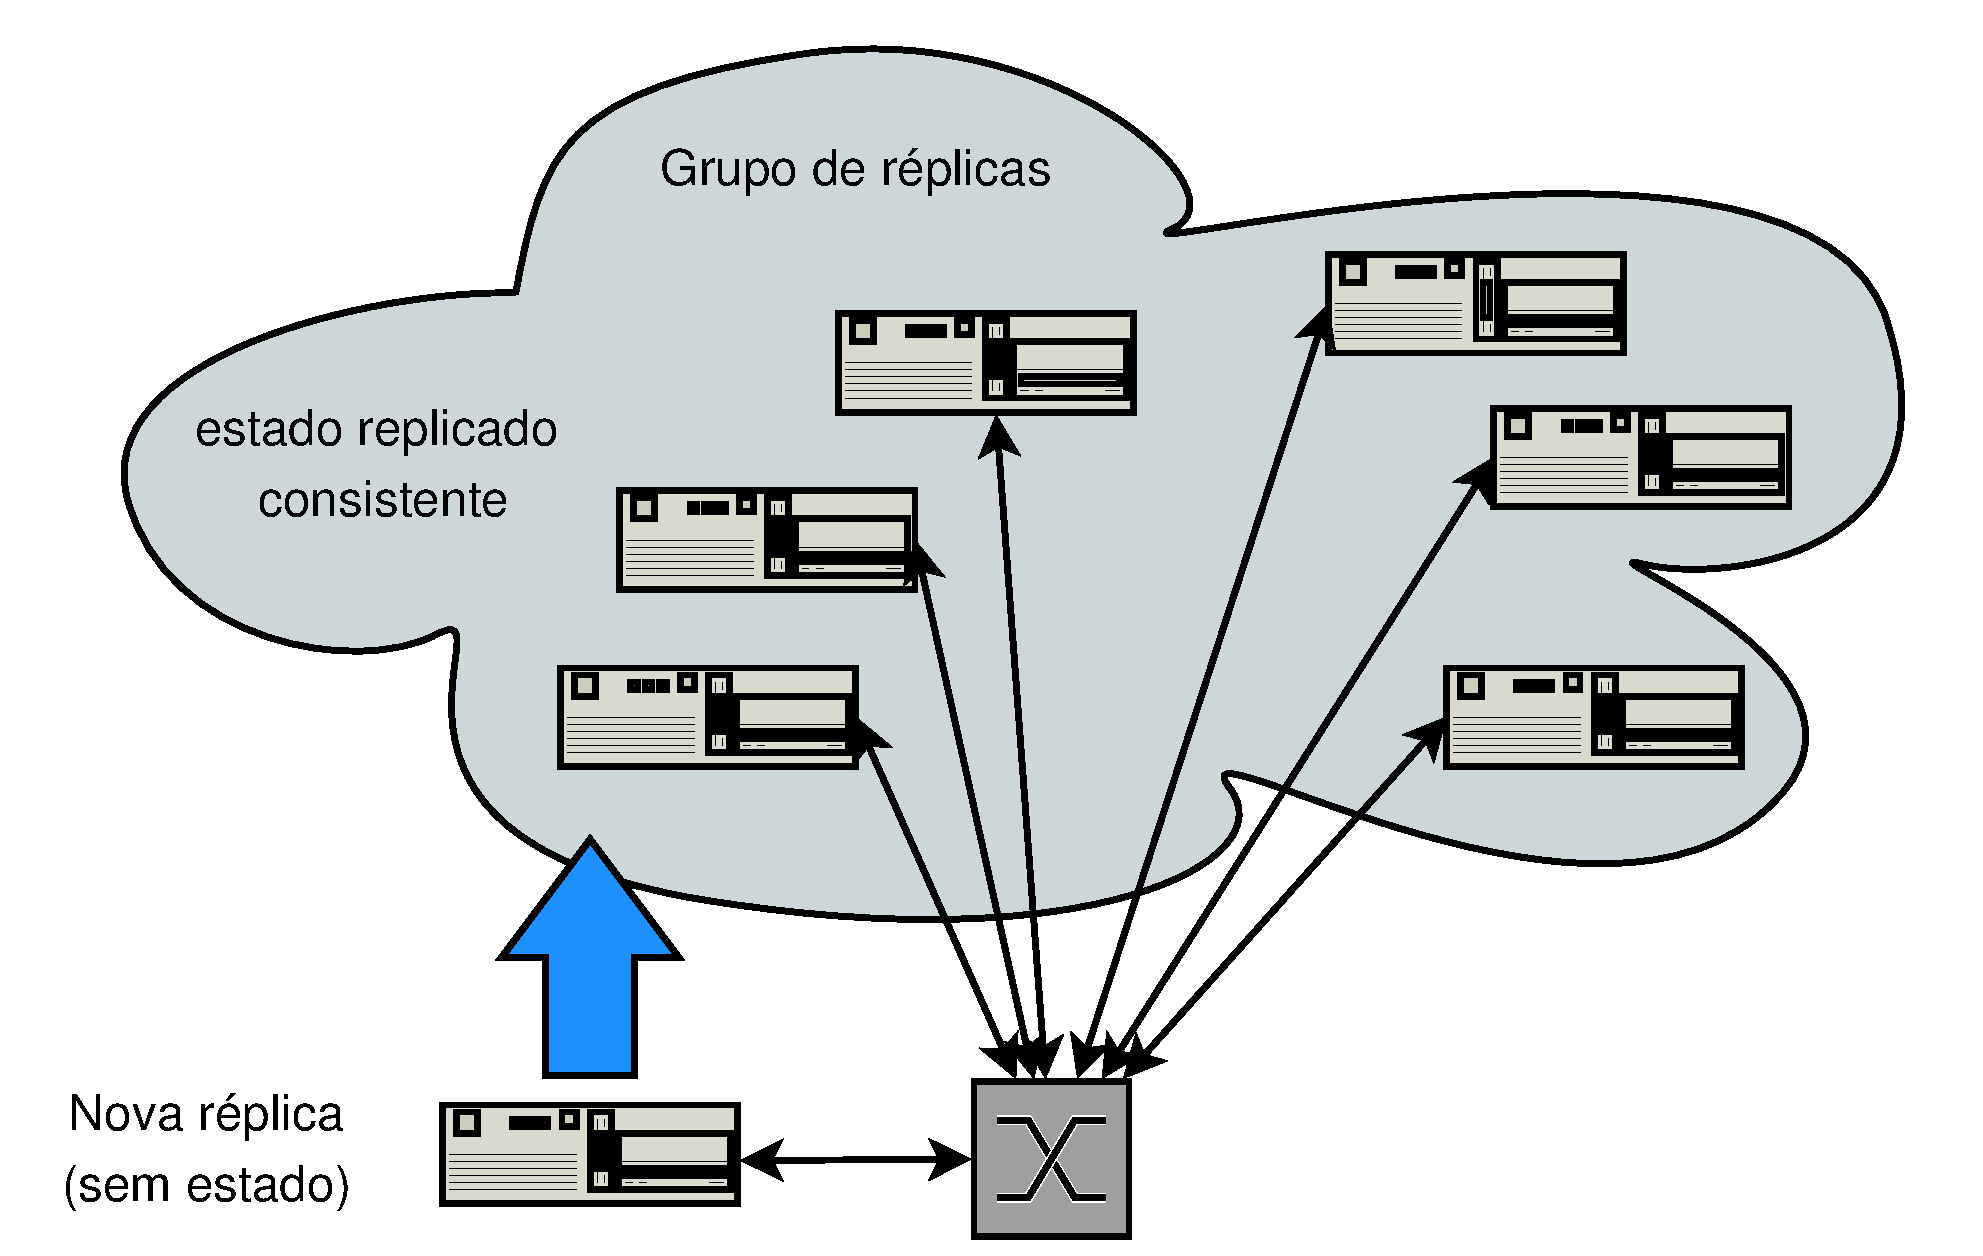
\includegraphics[width=11cm]{conteudo/capitulos/figuras/inclusao_replica_cluster.eps}
  \caption{Inclusão de réplica}
  \label{fig:inclusao}
\end{figure}

O mecanismo descrito na seção anterior deve ser regido por uma política de criação e
remoção de réplicas leitoras. A  motivação por trás da criação de réplicas leitoras é
permitir que o sistema reaja de forma autônoma a picos de carga sem comprometer o
desempenho do mesmo. No entanto, sem uma política cuidadosa de reconfiguração corre-se o
risco de gastar muitos dos recursos do sistema no próprio processo de reconfiguração,
anulando quaisquer ganhos advindos do acréscimo de novas réplicas leitoras.

A política de reconfiguração deve, desta forma, ser um equilíbrio entre o custo de se
instanciar uma nova réplica leitora e os ganhos de desempenho a serem auferidos após esta
instanciação. O trabalho de especificação de parâmetros para esta política ainda está em
seu estágio inicial, dependendo de estudos mais aprofundados para caracterizar os custos
envolvidos.

\subsection{Paxos com Réplicas Leitoras}\label{sec:replicas_leitoras}

A ideia principal da abordagem proposta é utilizar réplicas que não participem do processo
de decisão de instâncias de consenso. Isso é feito com a adoção de \emph{réplicas
leitoras}, que são réplicas onde apenas parte dos agentes do algoritmo Paxos estão
executando. Para maior clareza de exposição, quando necessário, chamaremos as réplicas
contendo todos os agentes ativos de \emph{réplicas votantes}. Para suportar a adaptação
elástica a novos perfis de desempenho, desenvolvemos um mecanismo para o
\emph{provisionamento de réplicas} e uma \emph{política de reconfiguração}.

\subsubsection{Réplicas Leitoras}

Réplicas leitoras são réplicas onde apenas os agentes proponente e aprendiz estão
executando. Dessa forma, do ponto de vista do conjunto de processos que implementam o
algoritmo Paxos, uma réplica leitora é capaz apenas de propor operações a serem aplicadas
no estado replicado e de aprender operações decididas pelo conjunto de receptores. Do
ponto de vista do cliente da aplicação replicada um réplica leitora se comporta como uma
réplica votante: ela atende requisições de qualquer tipo garantindo a execução atômica das
mesmas.

As réplicas leitoras não assumem um papel fundamental na execução do algoritmo Paxos, no
entanto elas se integram de forma consistente com a operação das réplicas votantes por
meio de suas funções fundamentais: propor e aprender requisições de escrita. As réplicas
leitoras propõem novas requisições a serem executadas em nome de seus clientes através de
seu agente proponente. O proponente encaminha a operação ao coordenador que por sua vez
decide, em conjunto com os receptores, a ordem da mesma através de uma rodada de Paxos,
como descrito no \autoref{cap1:replicacao_ativa_paxos}. Uma vez que a decisão é alcançada,
a mesma é difundida para o resto do sistema. Nesse momento o agente aprendiz da réplica
leitora toma conhecimento da decisão e atualiza o seu estado interno, sem a participação
ativa do coordenador ou de qualquer receptor.

Tanto o processo de proposta quanto o de aprendizado executado por uma réplica leitora
devem usar as mesmas estratégias de implementação das réplicas votantes. Na verdade, em
nossa implementação usando Treplica, as réplicas leitoras foram construídas a partir da
separação modular dos agentes que implementam Paxos. Dessa forma, reutilizamos os mesmos
componentes e por consequência essas réplicas são capazes de detectar e reenviar propostas
perdidas, detectar e corrigir lacunas na sequência de instâncias de consenso, fazer
controle de fluxo e de congestionamento, entre outras operações fundamentais para uma
operação eficiente de Paxos \cite{vieira-tr10b}.

Uma consequência importante do uso de réplicas leitoras é que essas réplicas,
consistentemente com as funções que elas assumem no algoritmo Paxos, não precisam de
memória persistente para sua operação. Isso se deve ao fato de que elas não executam as
Fases 1 e 2 do algoritmo. Porém, pode ser interessante que essas réplicas registrem a
proposta decidida de forma a não precisar realizar uma recuperação completa em caso de
falha. Na nossa proposta de réplicas leitoras decidimos não fazer esse registro de forma a
remover completamente a escrita em memória persistente do caminho crítico de execução. É
interessante observar que a escrita eliminada ocorre somente quando a réplica leitora
atualiza o seu estado de acordo com as propostas decididas pelos receptores das réplicas
votantes. Dessa forma, as réplicas leitoras conseguem manter seu estado atualizado com as
réplicas votantes com um custo mínimo. Elas também são capazes de processar requisições de
escrita com um custo similar àquele gerado pelas réplicas votantes ao executar as mesmas
requisições. Podemos argumentar que esse custo é menor, na medida que as réplicas leitoras
aliviam as réplicas votantes do custo de manter as conexões abertas com os clientes.

Utilizando réplicas leitoras, podemos formar grupos de réplicas com diferentes graus de
uso de memória persistente \cite{aguilera00}. Uma configuração simples seria mesclar
réplicas votantes e leitoras formando um conjunto híbrido de réplicas transparente para o
cliente, conforme ilustra a \autoref{fig:configuracao_replicas_leitoras} (a). É concebível
ainda uma configuração onde as réplicas votantes não entram em contato com os clientes,
sendo essa operação completamente delegada às replicas leitoras, configuração ilustrada
pela \autoref{fig:configuracao_replicas_leitoras} (b).

\begin{figure}[ht]
  \begin{center}
    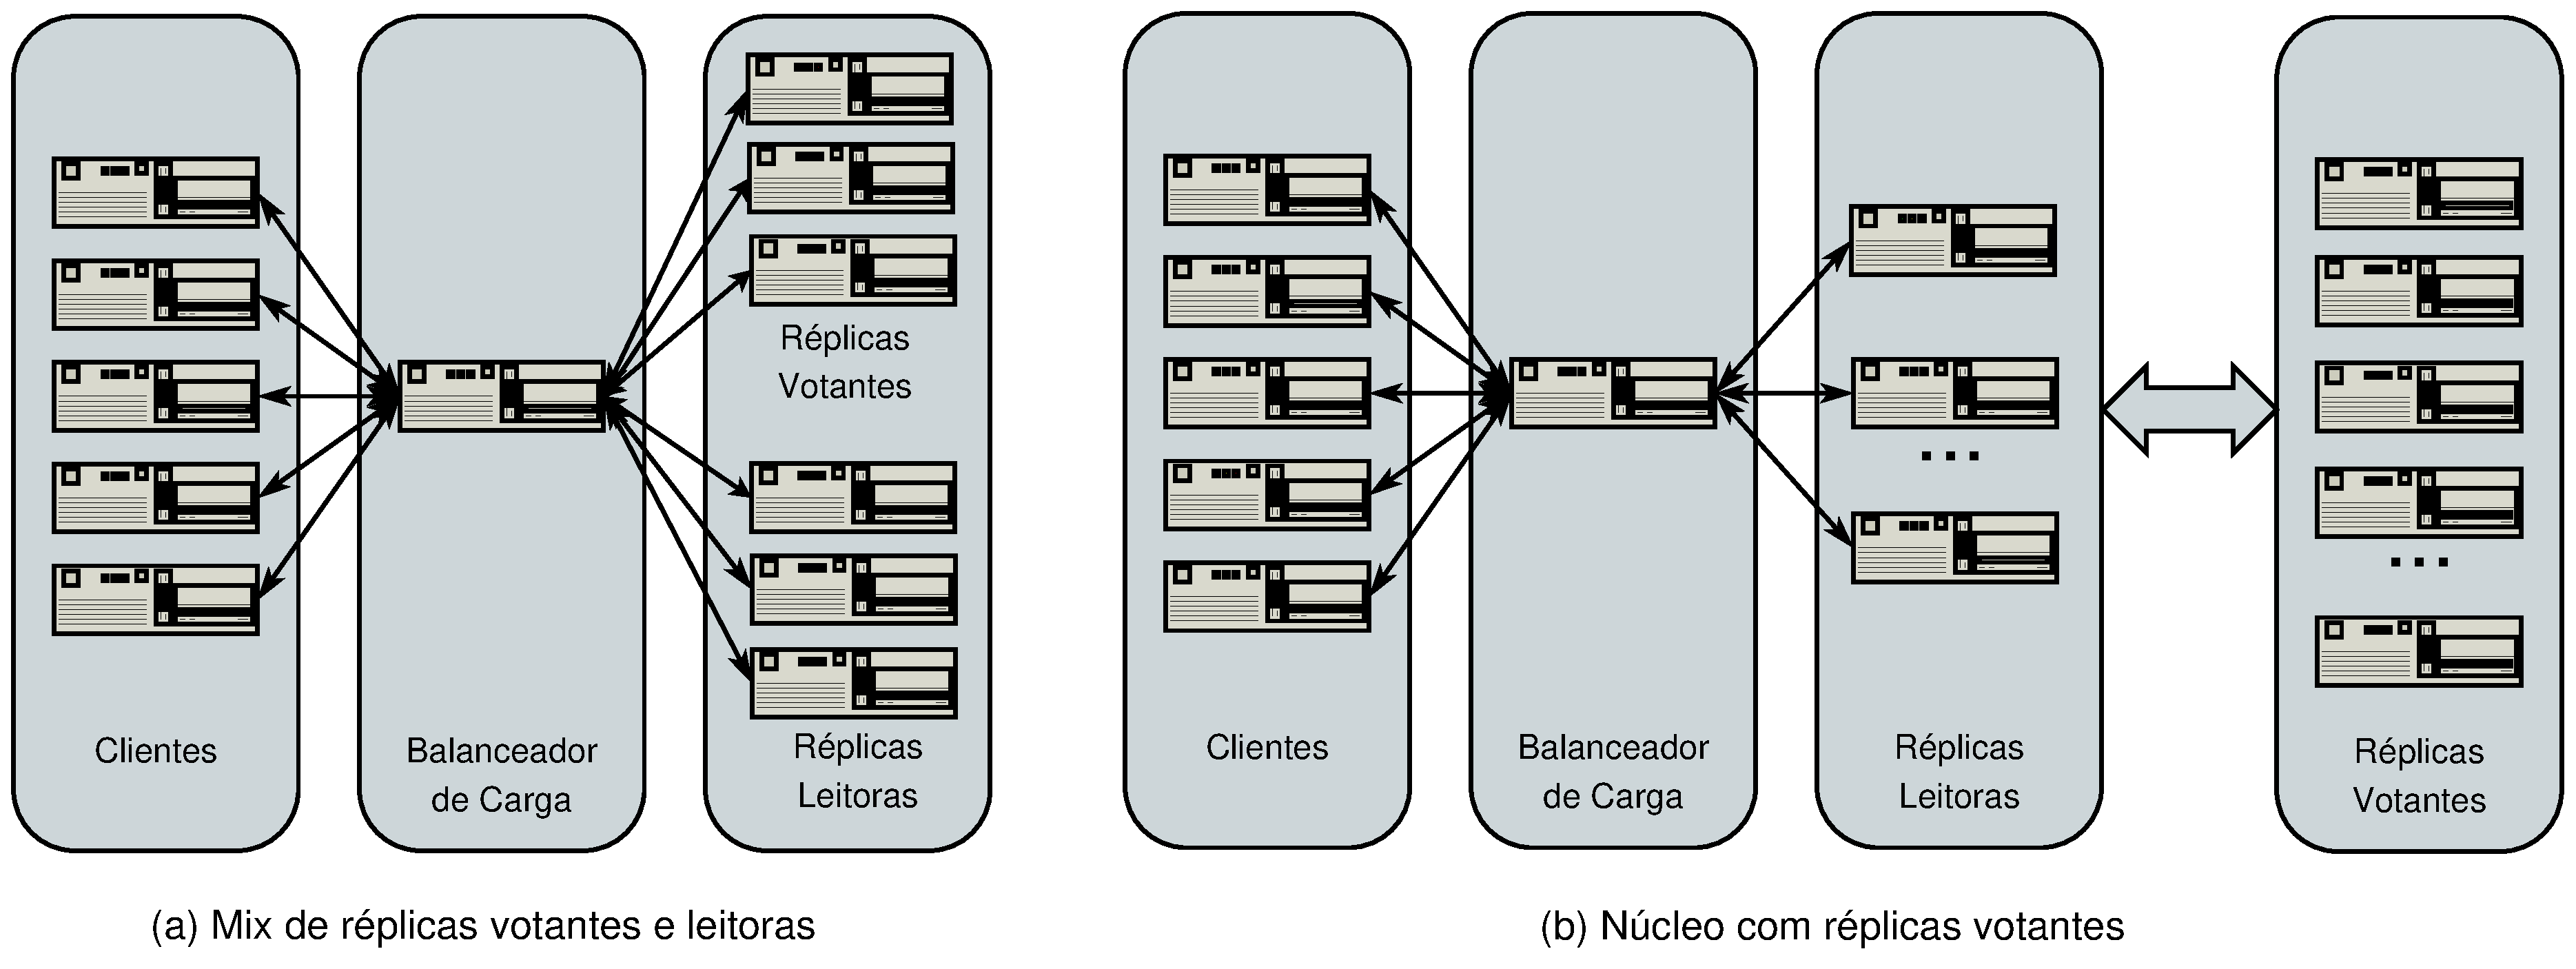
\includegraphics[width=16cm]{conteudo/capitulos/figuras/configuracao_replicas_leitoras.eps}
  \end{center}
  \caption{Configuração de Paxos com réplicas votantes e leitoras}
  \label{fig:configuracao_replicas_leitoras}
\end{figure}

As réplicas leitoras funcionam então como uma espécie de cache \emph{write-through}
distribuído. O estado replicado na memória destas réplicas permite atender diretamente as
requisições de leitura dos clientes, enquanto as requisições de escrita são repassadas ao
receptores. Podemos ver claramente que a taxa de acerto desse cache está diretamente
ligada à proporção de operações de leitura geradas pelos clientes e que a vazão de
operações de leitura tem o potencial de crescer linearmente com o número de réplicas
leitoras disponíveis.

\subsubsection{Componentes alterados}

Antes de detalharmos as alterações realizadas, vamos recapitular de forma resumida a
iteração entre os agentes de Paxos: proponentes enviam a sua proposta para o coordenador
que tenta alcançar consenso sobre a proposta em uma rodada, sendo que cada proposta
corresponde a uma ou mais requisições de escrita da aplicação sendo replicada.

Anteriormente, era possível uma única configuração de réplicas que empregava todos os
agentes de Paxos utilizando memória persistente. A nova funcionalidade de réplicas
leitoras foi implementada através de uma segregação modular dos agentes utilizados por uma
réplica votante:

\begin{itemize}
  \item Proponente: agente capaz de propor valores;
  \item Receptor: agente que vota em uma única proposta por rodada;
  \item Aprendiz: agente que aprende a decisão de consenso;
  \item Coordenador: agente responsável por garantir o funcionamento do algoritmo a cada
    rodada de consenso executada.
\end{itemize}

A classe denominada \classname{PaxosPersistentQueue} é responsável por implementar o
agrupamento de todos esses agentes, caracterizando assim uma réplica votante. Podemos
definir, do ponto de vista de uma Máquina Virtual Java (JVM), que uam réplica votante
possui como uma das suas \emph{threads} ativas o \emph{main loop} da classe
\classname{PaxosPersistentQueue}. Em contra partida, uma réplica leitora, executa o
\emph{main loop} da classe \classname{PaxosReadonlyQueue}. Essa classe, implementa somente
a agregação dos agentes proponente e aprendiz, sem a utilização de memória persistente.
Detalharemos nas próximas seções a implementação proposta para esse componente.

\subsubsubsection{PaxosReadonlyQueue}

A classe \classname{PaxosReadonlyQueue} foi criada para fornecer o mesmo comportamento da
classe \classname{PaxosPersistenteQueue}: disponibilizar uma fila que será utilizada pelo
protocolo Paxos. No entanto, as operações suportadas por \classname{PaxosReadonlyQueue}
não as mesmas. Do ponto de vista do processamento de mensagens postadas na fila, as
seguintes propriedades foram supostas para caracterizar uma réplica leitora:

\begin{itemize}
  \item Abdicar liderança: todas as mensagens relacionadas a eleição de líder não são
    processadas, logo é eliminada qualquer possibilidade de uma réplica leitora se tornar
    coordenadora de uma rodada de Paxos.
  \item Inelegível ao voto: mensagens relacionadas a votação de uma proposta são
    ignoradas. Dessa forma, réplicas leitoras não participam do processo de decisão de
    consenso e não são essenciais para o progresso do algoritmo Paxos.
  \item Aprendizado: todas as mensagens endereçadas ao componente \classname{Learner} são
    processadas pela fila. Consequentemente, os mecanismos descobrir qual foi o consenso
    de uma determinada rodada são habilitados.
\end{itemize}

O principal objetivo dessa classe é participar das operações que não exigem dados
persistentes para garantir correção do algoritmo, oferecendo instâncias capazes de atuar
parcialmente nas fases de Paxos. Do ponto de vista do cliente da aplicação um réplica
leitora se comporta como uma réplica votante: ela atende requisições de qualquer tipo
garantindo a execução atômica das mesmas. Sendo assim, as seguintes premissas não podem
ser violadas:

\begin{itemize}
  \item Mensagens quem alteram o estado (escrita): são resolvidas pelo aglomerado de
    réplicas orquestrado pelo protocolo Paxos, porém réplicas que não possuem grau de
    memória persistente não participam da decisão de consenso.
  \item Mensagens que não alteram estado (leitura): são resolvidas localmente independente
    do grau de memória da réplica.
\end{itemize}

Do ponto de vista de uma réplica votante, não é possível distinguir se a proposta é
oriunda de uma réplica votante ou leitora. O mecanismo para configuração do grau de
memória de uma réplica em Treplica atua de forma transparente junto com protocolo Paxos,
respeitando a forte premissa: o número de réplicas leitoras nunca deve afetar o número de
réplicas votantes. Sendo assim, podemos afirmar que o progresso e a correção do algoritmo
não são violados.

Réplicas oferecem um poder de manobra para aliviar a carga de processamento das réplicas
votantes com relação a mensagens de leituras, podendo ser configuradas de tal forma que
nenhuma mensagem de leitura seja processada por uma réplica votante. Avaliar e propor
soluções para configuração do conjunto de réplicas não faz parte do escopo desse trabalho.

\subsubsubsection{WeakSecretary}

<SNR>104_(count)A classe \classname{WeakSecretary} apresenta uma abstração de I/O sem persistência de
dados em disco. Esse componente é uma versão leve da classe \classname{Secretary}
(\autoref{subsec:secretary}), ela é utilizada pelos agentes de Paxos para enviar mensagens
pela rede, através do intermédio do componente \classname{Transport}
(\autoref{subsec:transport}). Essa classe foi projetada para trabalhar com dados somente
em memória, dessa forma todos os dados computados são perdidos na presença de defeitos na
réplica. No entanto, na ausência de falhas nos beneficiamos da eliminação de uma operação
custosa relacionada com I/O em disco.

\classname{WeakSecretary} também é responsável por lidar com o componente
\classname{Ledger} (\autoref{subsec:ledger}) e com a fila de objetos utilizada
para entregar mensagens para a camada da aplicação. A principal razão para a criação dessa
abstração em Treplica foi eliminar a operação de persistência em disco, gerando um
componente volátil, capaz de oferecer as operações essenciais para o progresso do
algoritmo sem o ônus da escrita em disco.

\subsubsection{Provisionamento de Réplicas Leitoras}

É possível utilizar os mecanismos tradicionais de Treplica para provisionar uma nova
réplica leitora. Em resumo, uma réplica que se integra ao sistema pela primeira vez ou
após uma falha demorada deve recuperar o seu estado. Esse processo acontece através de um
mecanismo de preenchimento de lacunas, que observa que não pode executar novas requisições
de escrita sem antes executar as requisições anteriores \cite{vieira-tr10b}. Esse
procedimento é voltado para reparar pequenas interrupções e não a recuperação do estado
completo de uma réplica. Em particular, no caso de uma réplica leitora sem estado
persistente, o tamanho dessa recuperação pode ser muito grande em termos do número de
\emph{requisições} a serem reexecutadas, pois ela sempre parte do estado inicial vazio.

Foi necessário então criar um procedimento de provisionamento de réplicas, de forma a
permitir o rápido início de uma réplica leitora. Esse mecanismo não é necessariamente
exclusivo de réplicas leitoras e pode ser aplicado a réplicas normais. Porém, neste
primeiro momento, ele tira proveito do fato dessas réplicas não terem memória persistente.
Em particular, a adição ou remoção de uma réplica leitora não altera o número de
receptores executando o algoritmo, não havendo necessidade de se realizar um
reconfiguração custosa \cite{lamport10}.

\subsection{Equalização de estado}

Treplica possui outro potencial candidato para empregar o protocolo de transferência: o
componente detector lacunas na sequência de instâncias de consenso. Lacunas podem surgir
por diferentes motivos: falha-e-recuperação na réplica, perda de mensagens ou ainda
réplicas com grandes diferenças de capacidade de processamento. Para preencher lacunas
detectadas, o componente solicita retransmissão da instância de consenso em uma
determinada rodada. É perceptível que na presença de grandes lacunas essa abordagem
exigirá uma longa sequência de retransmissões.

Para exemplificar o potencial problema do detector de lacunas, vamos supor que a aplicação
$x$ está passando por um grande pico de processamento (\emph{flash crowds}) e que a
réplica $r$ possui uma grande lacuna. O mecanismo detector de lacunas solicitará
retransmissão das instâncias de consenso não conhecidas por ele, aumentando a concorrência
no meio compartilhado pelas réplicas: a rede. Como solução alternativa, podemos utilizar o
mecanismo de transferência, para concentrar em uma única mensagem, o estado resultante das
aplicações das instâncias de consenso. Dessa forma, o novo mecanismo suposto para detectar
lacunas tem capacidade de:

\begin{itemize}
  \item Retransmissão de instância de consenso: utilizado para preencher pequenas lacunas
    na sequência de consenso.
  \item Protocolo de transferência de estado: utilizado para preencher grandes lacunas,
    onde retransmissão tem potencial perda de desempenho.
\end{itemize}

